\capitulo{RESULTADOS OBTIDOS}


\iniciocapitulo

Após o sistema implementado foram realizadas uma bateria de testes para que os valores paramêtros inicias fossem definidos, o dados utiliados tem  em sua composição o total de 10 salas e um curso com o total de 46 disciplinas e duas respectivas obrigatoriedades, serão utilizados como paramêtros iniciais os dados representados na Figura~\ref{fig:parametrosAg}, no caso uma população com 100 individuos, 60\% de croosover 20\% de mutação, e elitismos  estes dados foram tirados como base na conclusão do trabalho de \cite{deleonardo}. Os testes realizados tiveram uma maquina com a seguinte configuração, Intel(R) Core(TM) i5 3.40GHz com 16Gb de mémoria RAM sob o sistema operacional Windows 7 64bit.\par

\begin{figure}[!htb]
\caption[Parâmetros utilizados para o teste inicial]{Parâmetros utilizados para o teste inicial}
\label{fig:parametrosAg}
\centering
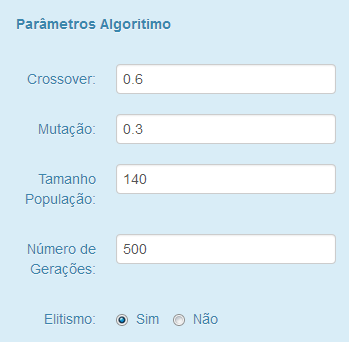
\includegraphics[scale=0.5]{imagens/parametrosDoAlgoritimo.png}
\\ \textbf{\footnotesize Fonte: Desenvolvido pelo autor}
\end{figure}

Gráfico com todos os parametros

Gráfico sem croossvoer

Gráfico sem mutação

Gráfico sem elitismo

Tempo de cada geração




Despois do sistema implementado		

Entrada processamento e saida

ajuste do algoritomo de alocação


falar do algoritimo que não evolui sem o crossover so com mutação.



\capitulo{CONSIDERAÇÕES FINAIS}

\iniciocapitulo

*Relembra ro problema e comprar como o resultadoo bjetido.

Discussão dos resultados obtidos na pesquisa, onde se verificam as observações pessoais do autor. Poderá também apresentar sugestões de novas linhas de estudo. A conclusão deve estar de acordo com os objetivos do trabalho. A conclusão não deve apresentar citações ou interpretações de outros autores.

\secao{Trabalhos futuros}

Criar um DW para geração dos relatorios de acordo com a dimensão escolhida.

Utilização de outros algoritimos para a resolução do problema ex. algoritimos evolutivos formiga entre outros.

Pegar o feed back do usuario para melhoria na interface, e do algoritimo.